% Options for packages loaded elsewhere
\PassOptionsToPackage{unicode}{hyperref}
\PassOptionsToPackage{hyphens}{url}
%
\documentclass[
]{book}
\usepackage{amsmath,amssymb}
\usepackage{lmodern}
\usepackage{iftex}
\ifPDFTeX
  \usepackage[T1]{fontenc}
  \usepackage[utf8]{inputenc}
  \usepackage{textcomp} % provide euro and other symbols
\else % if luatex or xetex
  \usepackage{unicode-math}
  \defaultfontfeatures{Scale=MatchLowercase}
  \defaultfontfeatures[\rmfamily]{Ligatures=TeX,Scale=1}
\fi
% Use upquote if available, for straight quotes in verbatim environments
\IfFileExists{upquote.sty}{\usepackage{upquote}}{}
\IfFileExists{microtype.sty}{% use microtype if available
  \usepackage[]{microtype}
  \UseMicrotypeSet[protrusion]{basicmath} % disable protrusion for tt fonts
}{}
\makeatletter
\@ifundefined{KOMAClassName}{% if non-KOMA class
  \IfFileExists{parskip.sty}{%
    \usepackage{parskip}
  }{% else
    \setlength{\parindent}{0pt}
    \setlength{\parskip}{6pt plus 2pt minus 1pt}}
}{% if KOMA class
  \KOMAoptions{parskip=half}}
\makeatother
\usepackage{xcolor}
\IfFileExists{xurl.sty}{\usepackage{xurl}}{} % add URL line breaks if available
\IfFileExists{bookmark.sty}{\usepackage{bookmark}}{\usepackage{hyperref}}
\hypersetup{
  pdftitle={Parcel-level metrics for evaluating housing sites},
  pdfauthor={Carole Voulgaris and Elizabeth Christoforetti},
  hidelinks,
  pdfcreator={LaTeX via pandoc}}
\urlstyle{same} % disable monospaced font for URLs
\usepackage{color}
\usepackage{fancyvrb}
\newcommand{\VerbBar}{|}
\newcommand{\VERB}{\Verb[commandchars=\\\{\}]}
\DefineVerbatimEnvironment{Highlighting}{Verbatim}{commandchars=\\\{\}}
% Add ',fontsize=\small' for more characters per line
\usepackage{framed}
\definecolor{shadecolor}{RGB}{248,248,248}
\newenvironment{Shaded}{\begin{snugshade}}{\end{snugshade}}
\newcommand{\AlertTok}[1]{\textcolor[rgb]{0.94,0.16,0.16}{#1}}
\newcommand{\AnnotationTok}[1]{\textcolor[rgb]{0.56,0.35,0.01}{\textbf{\textit{#1}}}}
\newcommand{\AttributeTok}[1]{\textcolor[rgb]{0.77,0.63,0.00}{#1}}
\newcommand{\BaseNTok}[1]{\textcolor[rgb]{0.00,0.00,0.81}{#1}}
\newcommand{\BuiltInTok}[1]{#1}
\newcommand{\CharTok}[1]{\textcolor[rgb]{0.31,0.60,0.02}{#1}}
\newcommand{\CommentTok}[1]{\textcolor[rgb]{0.56,0.35,0.01}{\textit{#1}}}
\newcommand{\CommentVarTok}[1]{\textcolor[rgb]{0.56,0.35,0.01}{\textbf{\textit{#1}}}}
\newcommand{\ConstantTok}[1]{\textcolor[rgb]{0.00,0.00,0.00}{#1}}
\newcommand{\ControlFlowTok}[1]{\textcolor[rgb]{0.13,0.29,0.53}{\textbf{#1}}}
\newcommand{\DataTypeTok}[1]{\textcolor[rgb]{0.13,0.29,0.53}{#1}}
\newcommand{\DecValTok}[1]{\textcolor[rgb]{0.00,0.00,0.81}{#1}}
\newcommand{\DocumentationTok}[1]{\textcolor[rgb]{0.56,0.35,0.01}{\textbf{\textit{#1}}}}
\newcommand{\ErrorTok}[1]{\textcolor[rgb]{0.64,0.00,0.00}{\textbf{#1}}}
\newcommand{\ExtensionTok}[1]{#1}
\newcommand{\FloatTok}[1]{\textcolor[rgb]{0.00,0.00,0.81}{#1}}
\newcommand{\FunctionTok}[1]{\textcolor[rgb]{0.00,0.00,0.00}{#1}}
\newcommand{\ImportTok}[1]{#1}
\newcommand{\InformationTok}[1]{\textcolor[rgb]{0.56,0.35,0.01}{\textbf{\textit{#1}}}}
\newcommand{\KeywordTok}[1]{\textcolor[rgb]{0.13,0.29,0.53}{\textbf{#1}}}
\newcommand{\NormalTok}[1]{#1}
\newcommand{\OperatorTok}[1]{\textcolor[rgb]{0.81,0.36,0.00}{\textbf{#1}}}
\newcommand{\OtherTok}[1]{\textcolor[rgb]{0.56,0.35,0.01}{#1}}
\newcommand{\PreprocessorTok}[1]{\textcolor[rgb]{0.56,0.35,0.01}{\textit{#1}}}
\newcommand{\RegionMarkerTok}[1]{#1}
\newcommand{\SpecialCharTok}[1]{\textcolor[rgb]{0.00,0.00,0.00}{#1}}
\newcommand{\SpecialStringTok}[1]{\textcolor[rgb]{0.31,0.60,0.02}{#1}}
\newcommand{\StringTok}[1]{\textcolor[rgb]{0.31,0.60,0.02}{#1}}
\newcommand{\VariableTok}[1]{\textcolor[rgb]{0.00,0.00,0.00}{#1}}
\newcommand{\VerbatimStringTok}[1]{\textcolor[rgb]{0.31,0.60,0.02}{#1}}
\newcommand{\WarningTok}[1]{\textcolor[rgb]{0.56,0.35,0.01}{\textbf{\textit{#1}}}}
\usepackage{longtable,booktabs,array}
\usepackage{calc} % for calculating minipage widths
% Correct order of tables after \paragraph or \subparagraph
\usepackage{etoolbox}
\makeatletter
\patchcmd\longtable{\par}{\if@noskipsec\mbox{}\fi\par}{}{}
\makeatother
% Allow footnotes in longtable head/foot
\IfFileExists{footnotehyper.sty}{\usepackage{footnotehyper}}{\usepackage{footnote}}
\makesavenoteenv{longtable}
\usepackage{graphicx}
\makeatletter
\def\maxwidth{\ifdim\Gin@nat@width>\linewidth\linewidth\else\Gin@nat@width\fi}
\def\maxheight{\ifdim\Gin@nat@height>\textheight\textheight\else\Gin@nat@height\fi}
\makeatother
% Scale images if necessary, so that they will not overflow the page
% margins by default, and it is still possible to overwrite the defaults
% using explicit options in \includegraphics[width, height, ...]{}
\setkeys{Gin}{width=\maxwidth,height=\maxheight,keepaspectratio}
% Set default figure placement to htbp
\makeatletter
\def\fps@figure{htbp}
\makeatother
\setlength{\emergencystretch}{3em} % prevent overfull lines
\providecommand{\tightlist}{%
  \setlength{\itemsep}{0pt}\setlength{\parskip}{0pt}}
\setcounter{secnumdepth}{5}
\usepackage{booktabs}
\usepackage{booktabs}
\usepackage{longtable}
\usepackage{array}
\usepackage{multirow}
\usepackage{wrapfig}
\usepackage{float}
\usepackage{colortbl}
\usepackage{pdflscape}
\usepackage{tabu}
\usepackage{threeparttable}
\usepackage{threeparttablex}
\usepackage[normalem]{ulem}
\usepackage{makecell}
\usepackage{xcolor}
\ifLuaTeX
  \usepackage{selnolig}  % disable illegal ligatures
\fi
\usepackage[]{natbib}
\bibliographystyle{plainnat}

\title{Parcel-level metrics for evaluating housing sites}
\author{Carole Voulgaris and Elizabeth Christoforetti}
\date{}

\begin{document}
\maketitle

{
\setcounter{tocdepth}{1}
\tableofcontents
}
\hypertarget{introduction}{%
\chapter{Introduction}\label{introduction}}

\hypertarget{motivation}{%
\chapter{Motivation}\label{motivation}}

Motivation for the project.

\hypertarget{related-work}{%
\chapter{Related work}\label{related-work}}

Talk about various area-level metrics

\begin{itemize}
\tightlist
\item
  Sprawl index
\item
  Neighborhood typology
\end{itemize}

Talk about VMT site work

\hypertarget{methodology}{%
\chapter{Methodology}\label{methodology}}

\hypertarget{variables}{%
\subsection{Variables}\label{variables}}

\hypertarget{categories-that-would-be-useful-things-to-predict}{%
\subsubsection{Categories that would be useful (things to predict?)}\label{categories-that-would-be-useful-things-to-predict}}

Owner-occupied?
Investor-owned?
Vacant?
Demolition in the past year (no construction since)
Construction in the past year

\hypertarget{factor-analysis-variables}{%
\subsubsection{factor analysis Variables}\label{factor-analysis-variables}}

The variables made it into the initial factor analysis were:

\begin{itemize}
\item
  Accessibility

  \begin{itemize}
  \tightlist
  \item
    Distance to transit (use number of transit stops within 1/2 mile walkshed)
  \item
    Share of old/new homes (use average age of homes within 1/2 mile walkshed)
  \item
    Transit frequency (use transit stops per hour within 1/2 mile walkshed)
  \end{itemize}
\item
  Affordability

  \begin{itemize}
  \tightlist
  \item
    Average Condition of homes in half-mile walkshed
  \item
    Median rent of block-groups with centroids within 1/2 mile walkshed.
  \item
    Median income of block groups with centroids within 1/2 mile walkshed.
  \item
    Median ownership cost of block groups with centroids within 1/2 mile walkshed.
  \end{itemize}
\item
  Close

  \begin{itemize}
  \tightlist
  \item
  \end{itemize}
\item
  Diverse buildings

  \begin{itemize}
  \tightlist
  \item
    Entropy of housing types (apartment, townhomes, etc) within 1/2 mile walkshed
  \end{itemize}
\item
  Other

  \begin{itemize}
  \tightlist
  \item
    Standard deviation of building age within 1/2 mile walkshed
  \end{itemize}
\end{itemize}

\hypertarget{data}{%
\section{Data}\label{data}}

We obtained data on property addresses, land uses, assessed values (for both
land and buildings), and the dates and prices of as many as the three
most-recent sales from\\
\citet{allegheny_county_office_of_property_assessments_allegheny_2022}, which
includes information on 582,116 properties in Allegheny County.

We also obtained latitude and longitude coordinates for each property from a
geocoder file provided by \citet{western_pennsylvania_regional_data_center_geocoders_2021}.
Over 99.5 percent of properties included in the assessment dataset are included
in the geocoder file. Properties without geocoded locations are excluded from
our analysis.

Potential development sites were identified as those

\begin{enumerate}
\def\labelenumi{\arabic{enumi}.}
\tightlist
\item
  classified as ``residential''
  (indicating residential properties with one to four housing units) or ``commercial''
  (which includes mixed-use developments and residential properties with more than four
  housing units), and
\item
  with a land use description in one of 59 possible categories\footnote{One site (3008 Phillip Dr in Clairton) is missing a land use description in the assessment data. We checked this address on Zillow to determine that this is a single-family home and classified it as such in our data.}. The most common of
  these are listed Table \ref{tab:list-site-uses}.\footnote{The land use descriptions that were
    classified as potential development sites but are not listed in Table
    \ref{tab:list-site-uses}, which combine to represent less than one percent of all sites
    are ``RIGHTOF WAY - RESIDENTIAL'', ``CONDOMINIUM UNIT'', ``DWG USED AS OFFICE'',
    ``APART:20-39 UNITS'', ``CONDO GARAGE UNITS'', ``COMMON AREA'', ``CONDO DEVELOPMENTAL
    LAND'', ``CONDEMNED/BOARDED-UP'', ``CONDOMINIUM OFFICE BUILDING'', ``INDEPENDENT LIVING
    (SENIORS)'', ``DWG USED AS RETAIL'', ``OTHER COMMERCIAL'', ``MOBILE HOMES/TRAILER PKS'',
    ``RIGHT OF WAY - COMMERCIAL'', ``GROUP HOME'', ``TOTAL/MAJOR FIRE DAMAGE - COMM'',
    ``OTHER COMMERCIAL HOUSING'', ``TOTAL/MAJOR FIRE DAMAGE'', ``COMM APRTM CONDOS 5-19
    UNITS'', ``MUNICIPAL URBAN RENEWAL'', ``COMMERCIAL LAND'', ``CAMPGROUNDS'', ``COMMON AREA
    OR GREENBELT'', ``CHARITABLE EXEMPTION/HOS/HOMES'', ``INCOME PRODUCING PARKING LOT'',
    ``DWG APT CONVERSION'', ``\textgreater10 ACRES VACANT'', ``MINOR FIRE DAMAGE'', ``COMM APRTM CONDOS
    20-39 UNITS'', ``COMMERCIAL/UTILITY'',
    ``H.O.A RECREATIONS AREA'', ``COMM APRTM CONDOS 40+ UNITS'', ``MINOR FIRE DAMAGE - COMM'',
    ``OTHER'', ``OTHER RESIDENTIAL STRUCTURE'', ``OWNED BY METRO HOUSING AU'', ``RESIDENTIAL VACANT
    LAND'', ``HUD PROJ \#221'', and ``VACANT LAND 0-9 ACRES''}.
\end{enumerate}

\begin{table}

\caption{\label{tab:list-site-uses}Most common land uses categorized as potential sites}
\centering
\begin{tabu} to \linewidth {>{\raggedright}X>{\raggedleft}X>{\raggedleft}X>{\raggedleft}X}
\toprule
USEDESC & Number of potential sites & Percent of potential sites & Cumulative percent of potential sites\\
\midrule
SINGLE FAMILY & 370,513 & 73.2 & 73.2\\
VACANT LAND & 62,672 & 12.4 & 85.5\\
TWO FAMILY & 17,293 & 3.4 & 89.0\\
TOWNHOUSE & 14,670 & 2.9 & 91.8\\
ROWHOUSE & 11,082 & 2.2 & 94.0\\
\addlinespace
VACANT COMMERCIAL LAND & 5,817 & 1.1 & 95.2\\
THREE FAMILY & 3,968 & 0.8 & 96.0\\
RES AUX BUILDING (NO HOUSE) & 3,601 & 0.7 & 96.7\\
RETL/APT'S OVER & 3,354 & 0.7 & 97.3\\
COMM AUX BUILDING & 2,825 & 0.6 & 97.9\\
\addlinespace
APART: 5-19 UNITS & 2,771 & 0.5 & 98.4\\
FOUR FAMILY & 2,058 & 0.4 & 98.9\\
BUILDERS LOT & 1,230 & 0.2 & 99.1\\
PARKING GARAGE/LOTS & 891 & 0.2 & 99.3\\
OFFICE/APARTMENTS OVER & 854 & 0.2 & 99.4\\
\addlinespace
MOBILE HOME & 666 & 0.1 & 99.6\\
APART:40+ UNITS & 529 & 0.1 & 99.7\\
DWG USED AS OFFICE & 440 & 0.1 & 99.8\\
APART:20-39 UNITS & 400 & 0.1 & 99.8\\
CONDEMNED/BOARDED-UP & 132 & 0.0 & 99.9\\
\bottomrule
\end{tabu}
\end{table}

Potential building sites were further filtered to exclude those with missing data
on the most recent sale (about one percent of all sites).\footnote{Four sites had sales
  prices listed that were unreasonably high. 3039 Liberty Avenue in Pittsburgh is
  listed as having sold for \$511,945,000 on August 30, 2021. Zillow lists this
  property as having sold on that date for \$511,945
  (\url{https://www.zillow.com/homedetails/3039-W-Liberty-Ave-Pittsburgh-PA-15216/2070262638_zpid/}, accessed 5/4/2022),
  so the value was corrected for what appears to have been a typo. 220 Hyeholde Dr
  in Coraopolis is listed as having sold for \$28,100,000 in 1967. This may also
  be a typo, and it also does not seem to be the most recent sale. Zillow lists
  this home as having sold for \$350,000 in 2004
  (\url{https://www.zillow.com/homes/220-hyeholde-dr,-Coraopolis,-PA_rb/11552817_zpid/},
  accessed 5/4/2022), so the data was corrected to add that as the most recent sale.
  Two other sites were identified as having unreasonably high sales values: 1339
  Arlington Avenue in Pittsburgh is a three-bedroom single-family home that is
  listed as having sold for \$57,010,813 in 1976 and a 0.06-acre vacant lot with
  tax ID 0165G00270000000 is listed as having sold for \$24,920,232 in 1936. The
  sales data for these sites were treated as missing.} for a total of\\
potential sites.

The focus of this analysis is on potential development sites rather than on
properties. Some properties in the assessor dataset are condominums where
multiple properties share a single parcel of land. We aggregated these to the
site level by identifying all properties with an assessed building value
greater than zero, a land value of zero, and a land use description that did
not indicate the land was vacant. If multiple such properties share an address,
we classified all properties at that address as a condominium and aggregated
them to the parcel level. This led to a final sample of 518,032 sites.

\hypertarget{tax-assessment-data}{%
\subsection{Tax assessment data}\label{tax-assessment-data}}

Three variables (total assessed fair market value, assessed fair market value of the building, and lot area) were taken directly from the county tax assessment data for use in our analysis. We also included the most recent listed sales price, adjusted for inflation.

To aggregate properties identified as condominiums to the site level, we summed
the total values for lot area, assessed land value, assessed building value, and
inflation-adjusted sale price. We log-transformed these four variables prior to
including them in our analysis. Their distributions are shown in
Figure \ref{fig:assessor-hist}.

\begin{figure}
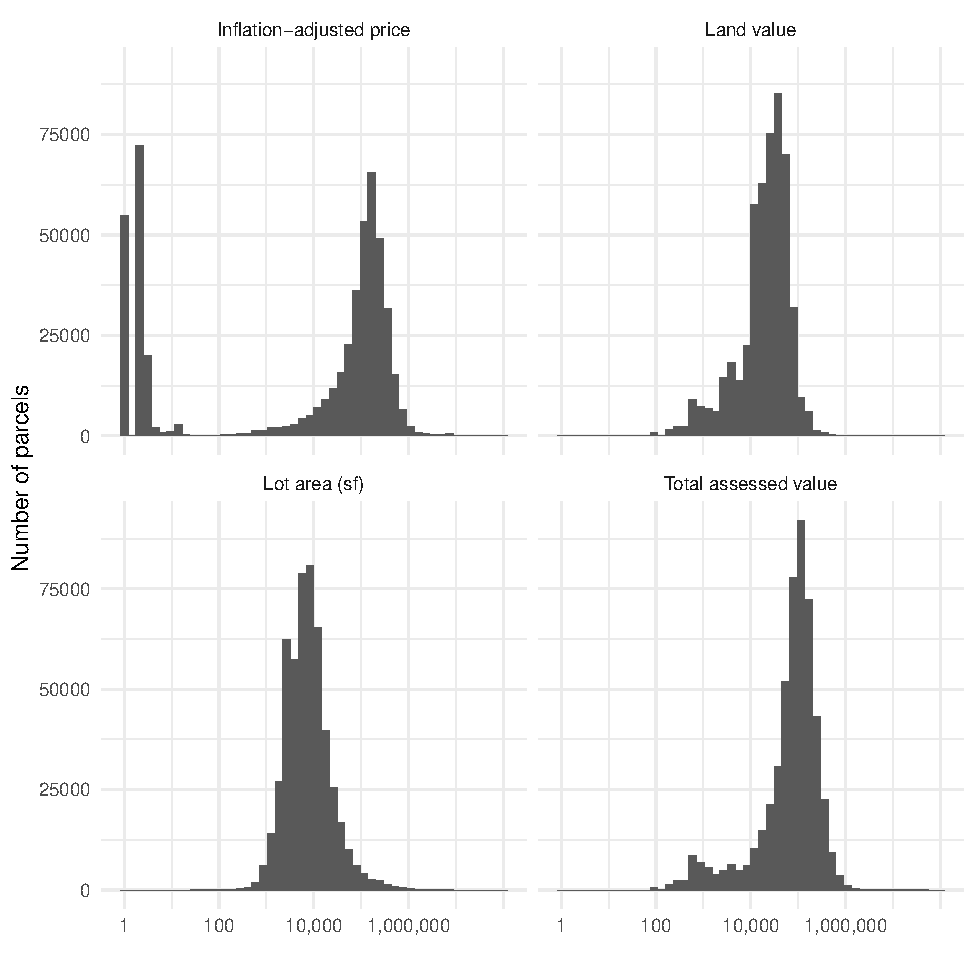
\includegraphics[width=1\linewidth]{_main_files/figure-latex/assessor-hist-1} \caption{Distribution of variables from tax assessor database}\label{fig:assessor-hist}
\end{figure}

\hypertarget{accessibilty-data}{%
\subsection{Accessibilty data}\label{accessibilty-data}}

Accessibilty was calculated from each of the 518,032 sites in our sample to
each of several location types described below.

\hypertarget{destination-parcels}{%
\subsubsection{Destination parcels}\label{destination-parcels}}

We used land use codes from the county assessor parcel data to identify
\emph{destination parcels} that residents might value access to. The most common
land use codes of identified destination parcels are listed in Table \ref{tab:dest-uses}.

\begin{table}

\caption{\label{tab:dest-uses}Land uses identified as potential destinations}
\centering
\begin{tabu} to \linewidth {>{\raggedright}X>{\raggedleft}X>{\raggedleft}X>{\raggedleft}X}
\toprule
USEDESC & Number of identified destinations & Percent of identified destinations & Cumulative percent of identified destinations\\
\midrule
MUNICIPAL GOVERNMENT & 10,376 & 29.88 & 29.88\\
CHURCHES, PUBLIC WORSHIP & 1,946 & 5.60 & 35.49\\
COMMERCIAL GARAGE & 1,735 & 5.00 & 40.48\\
OFFICE - 1-2 STORIES & 1,649 & 4.75 & 45.23\\
SMALL DETACHED RET(UNDER 10000) & 1,646 & 4.74 & 49.97\\
\addlinespace
OFFICE/WAREHOUSE & 1,386 & 3.99 & 53.96\\
COUNTY GOVERNMENT & 1,287 & 3.71 & 57.67\\
WAREHOUSE & 1,252 & 3.61 & 61.27\\
OWNED BY BOARD OF EDUCATION & 1,086 & 3.13 & 64.40\\
TOWNSHIP GOVERNMENT & 855 & 2.46 & 66.86\\
\addlinespace
LIVESTOCK O/T D \& P-CAUV & 805 & 2.32 & 69.18\\
LIGHT MANUFACTURING & 799 & 2.30 & 71.48\\
PUBLIC PARK & 710 & 2.04 & 73.53\\
RESTAURANT, CAFET AND/OR BAR & 697 & 2.01 & 75.54\\
GENERAL FARM & 607 & 1.75 & 77.28\\
\addlinespace
OWNED BY COLLEGE/UNIV/ACADEMY & 458 & 1.32 & 78.60\\
MEDICAL CLINICS/OFFICES & 445 & 1.28 & 79.88\\
RETL/OFF OVER & 442 & 1.27 & 81.16\\
OFFICE-ELEVATOR -3 + STORIES & 412 & 1.19 & 82.34\\
LODGE HALL/AMUSEMENT PARK & 386 & 1.11 & 83.46\\
\addlinespace
AUTO SALES \& SERVICE & 363 & 1.05 & 84.50\\
RETL/STOR OVER & 344 & 0.99 & 85.49\\
CEMETERY/MONUMENTS & 340 & 0.98 & 86.47\\
STATE GOVERNMENT & 331 & 0.95 & 87.42\\
CONVENIENCE STORE/GAS & 304 & 0.88 & 88.30\\
\bottomrule
\end{tabu}
\end{table}

\hypertarget{job-locations}{%
\subsubsection{Job locations}\label{job-locations}}

We identified \emph{job locations} based on data from a Longitudinal
Employer-Household Dynamics (LEHD) dataset published by the United States Census
Bureau \citep{united_states_census_bureau_lehd_2021}. The LEHD dataset provides the
total number of jobs in each census block in the United States, based on
employment tax records. The location of each job was defined as the centroid of
the block in which it was located. We downloaded job location data for
Pennsylvania and filtered it to include locations in the Pittsburgh metropolitan
area (Allegheny, Armstrong, Beaver, Butler, Fayette, Washington, and
Westmoreland counties).

In addition to calculating the accessibility to jobs of all categories, we also
calculated accessibility to several subsets of jobs. We disaggregated jobs by
earnings, reasoning that the usefulness of a job might vary depending on how
well it matches a workers skills or wage expectations. \emph{High-paying job locations}
are a subset of job locations where the worker earns more than \$3333 per month.
\emph{Low-paying job locations} are those where the worker earns \$1250 per month or less.

We also disaggregated jobs based on employment industry, based on the North
American Industry Classification System (NAICS), reasoning that the presence of
jobs particular industries might represent a shopping or recreation destination.
\emph{Retail job locations} are a subset of job locations in NAICS sector 44-45
(retail trade); \emph{Entertainment job locations} are those in NAICS sector 71
(arts, entertainment, and recreation); and \emph{Hospitality job locations} are
those in NAICS sector 72 (accommodation and food services).

Finally, we identified three location types that correspond with common non-work
trips: schools, grocery stores, and parks. \emph{Grocery store locations} were
identified as vendors participating in the Supplemental Nutrition Program for
Women, Infants, and Children (WIC). WIC vendor locations and \emph{school locations}
were obtained from the Allegheny County GIS portal
\citep{allegheny_county_office_of_information_technology_allegheny_2018, allegheny_county_office_of_information_technology_allegheny_2020}.
\emph{Park locations} were taken from the Pennsylvania Geospatial Data Clearinghouse
\citep{pennsylvania_department_of_conservation_and_natural_resources_pennsylvania_2015}.
Park locations were downloaded for Pennsylvania and filtered to Allegheny county.

We used the r5r package in the R programming language \citep{pereira_r5r_2021} to
calculate accessibility each destination type described above,
for each of four transportation modes (walking, cycling, driving, and transit).
The r5r package calculates accessibility as the weighted total number of
destinations reachable by a given mode, where destinations are weighted
according to a decay function, such that destinations that can be reached within
less time are assigned greater weight. We used a logistic decay function, as
illustrated in \ref{fig:show-decay-func}. For motorized modes, the decay
function had a mean (inflection) of 40 minutes and a standard deviation of 10
minutes. For non-motorized modes, the decay function had a mean of 20 minutes
and a standard deviation of 5 minutes.

\begin{figure}

{\centering 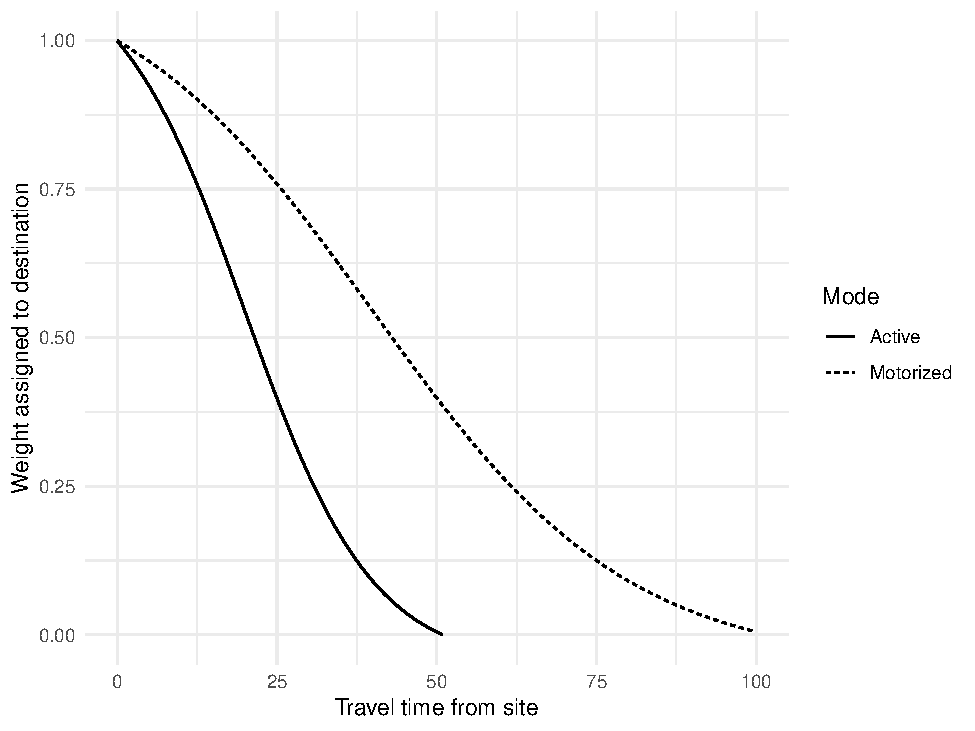
\includegraphics[width=0.8\linewidth]{_main_files/figure-latex/show-decay-func-1} 

}

\caption{Decay functions for accessibility calculations}\label{fig:show-decay-func}
\end{figure}

Calculating accessibility metrics for a combination of four transportation
modes and ten destination types yields 40 different accessibility variables. \ref{fig:show-decay-func}
illustrates the distributions of each of these variables.

\begin{figure}

{\centering 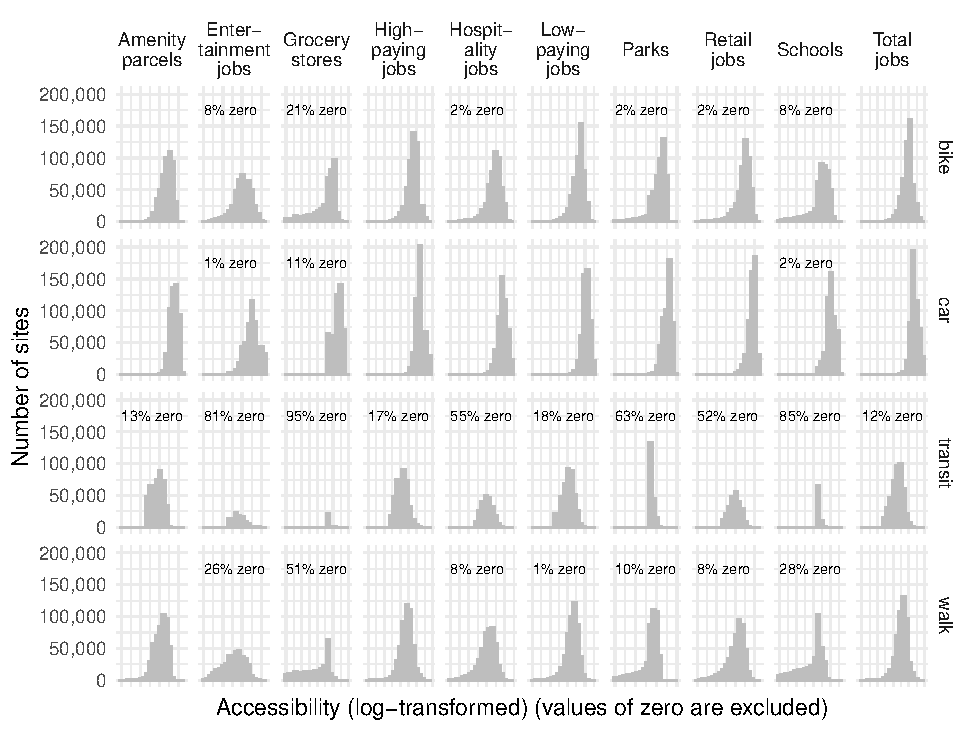
\includegraphics[width=1\linewidth]{_main_files/figure-latex/access-dist-1} 

}

\caption{Distributions of accessibility variables}\label{fig:access-dist}
\end{figure}

\hypertarget{disamenity-proximity}{%
\subsection{Disamenity proximity}\label{disamenity-proximity}}

We categorized several land uses in the county assessor data as
disamenities. The land use codes we used to identify disamenities are
listed in \ref{tab:bad-use-list}\footnote{289 properties related to coal mining
  (with land use descriptions of either ``COAL RIGHTS, WORKING INTERESTS'' or
  ``COAL LAND, SURFACE RIGHTS'') are co-located and are treated as a single
  site.}.

We included a disamenity proximity index in our analysis that we calculated
as the logarithm of the average distance from each site to the ten closest
disamenity sites. The distribution of this index is shown in \ref{fig:bad-prox}.

\begin{figure}

{\centering 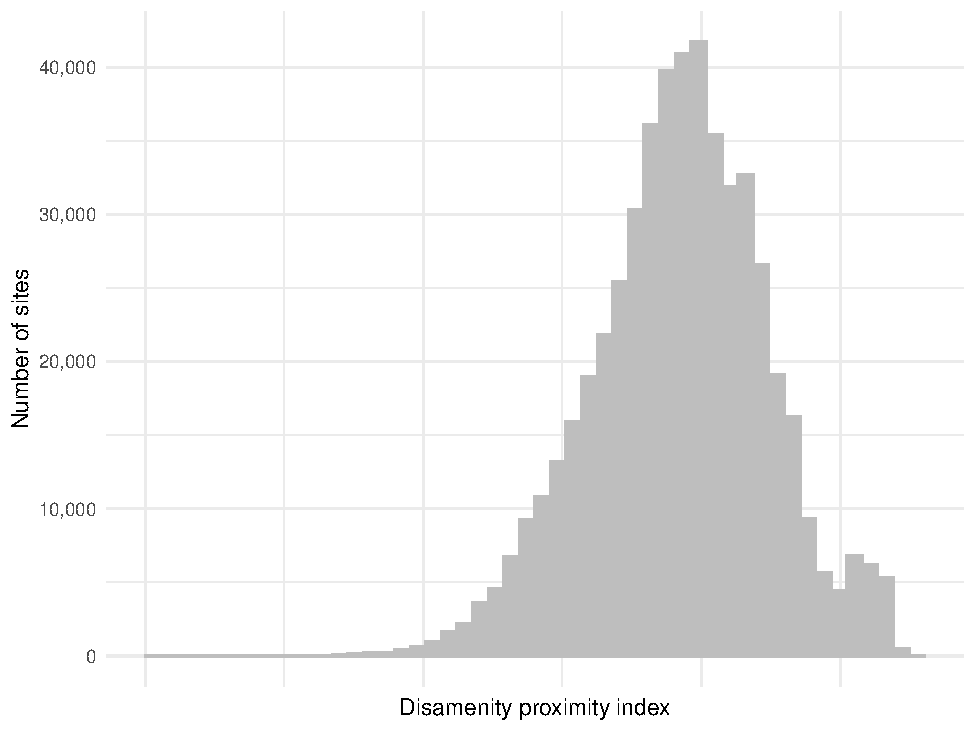
\includegraphics[width=0.8\linewidth]{_main_files/figure-latex/bad-prox-1} 

}

\caption{Distribution of average distance to nearest ten disamenity sites}\label{fig:bad-prox}
\end{figure}

\hypertarget{density}{%
\subsection{Density}\label{density}}

To represent the residential density around each site, we used the sf \citep{sf}, nngeo
\citep{nngeo} and tidycensus \citep{tidycensus} R packages to determine the smallest circular
buffer around each site containing a population of at least two thousand people,
based on the 2020 census. In denser places, a buffer with a smaller radius would
encompass two thousand residents. In more sparsely-populated places, a buffer
containing two thousand residents would be larger. The distribution of radii for
two-thousand-person site buffers is shown in \ref{fig:radii}.

\begin{figure}

{\centering 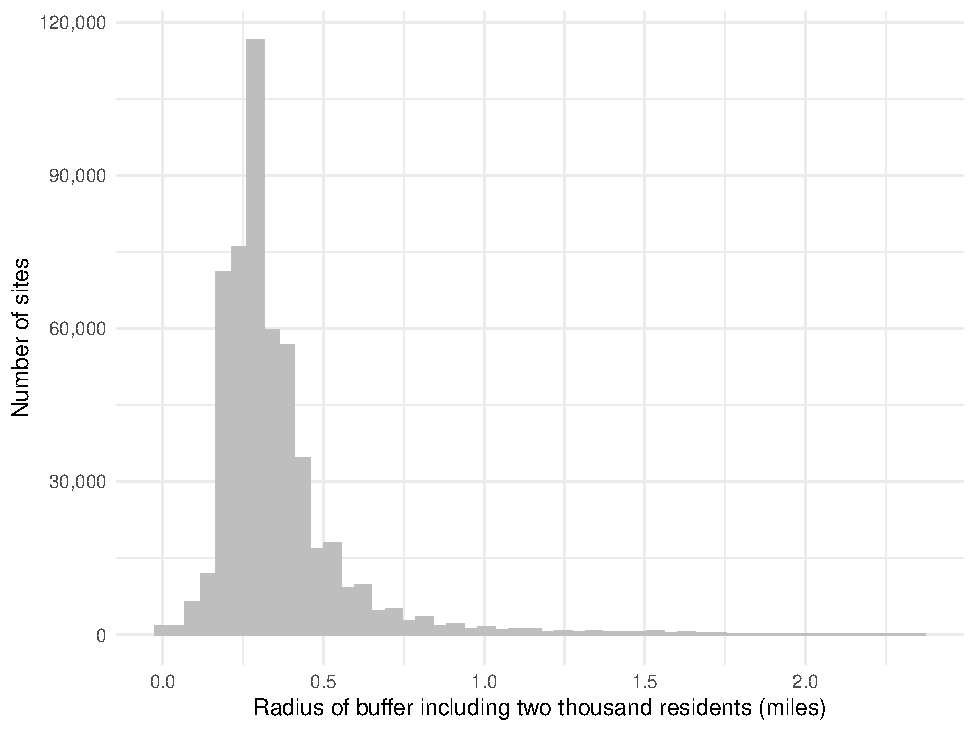
\includegraphics[width=0.8\linewidth]{_main_files/figure-latex/radii-1} 

}

\caption{Histogram of radii of buffer containing 2000 residents}\label{fig:radii}
\end{figure}

\hypertarget{population-diversity}{%
\subsection{Population diversity}\label{population-diversity}}

The two-thousand-resident buffers described above were also used as a basis to
estimate the racial diversity of residents in the immediate vicinity. For each
buffer, we calculated the percentage of residents that who identified in the 2020
census as non-Hispanic white, non-Hispanic Black, and Hispanic. The distributions
of these variables are shown in \ref{fig:divers-hist}.

\begin{figure}

{\centering 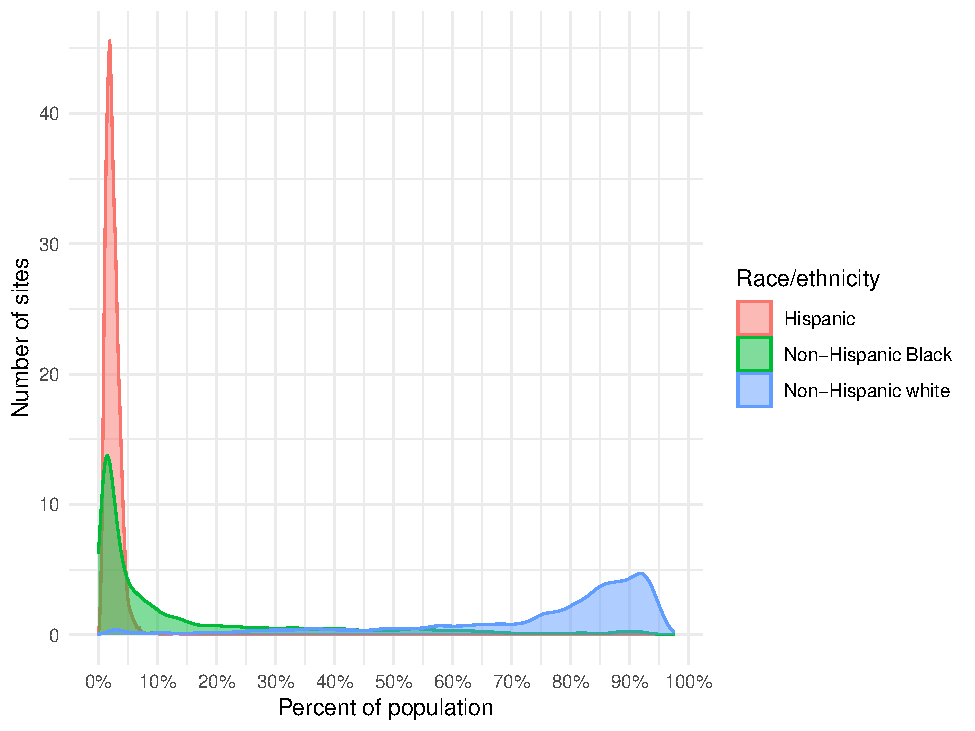
\includegraphics[width=0.8\linewidth]{_main_files/figure-latex/divers-hist-1} 

}

\caption{Histograms of population diversity variables}\label{fig:divers-hist}
\end{figure}

\hypertarget{land-use-diversity}{%
\subsection{Land use diversity}\label{land-use-diversity}}

We also calculated the total number of different land uses within each
two-thousand-resident buffer and used this as a measure of land-use diversity.
\ref{fig:land-divers}.

\begin{figure}

{\centering 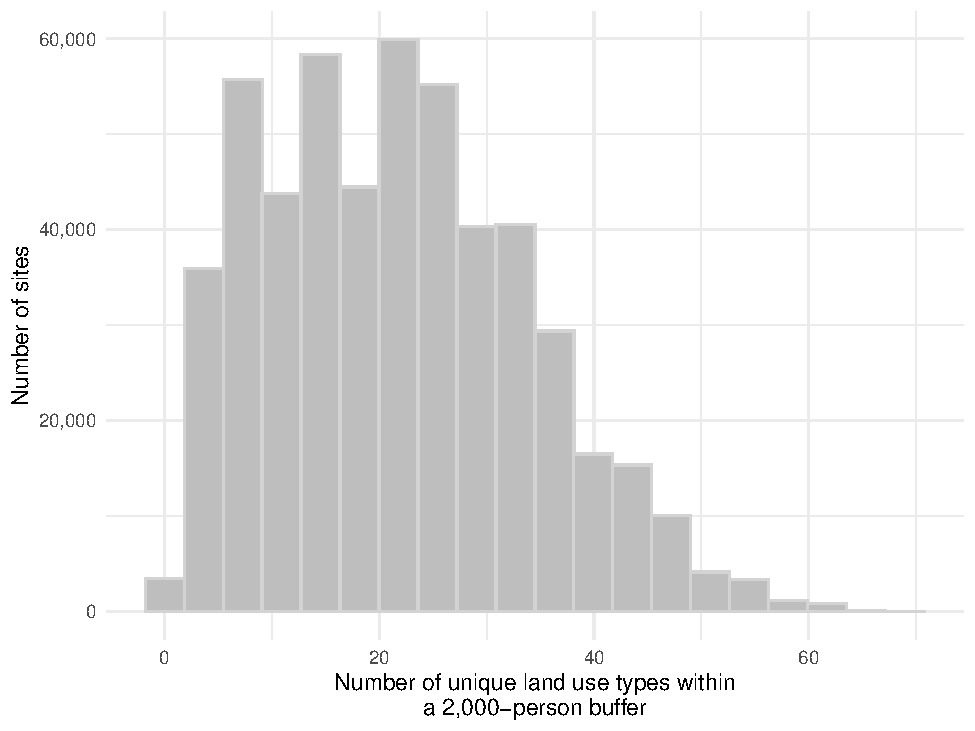
\includegraphics[width=0.8\linewidth]{_main_files/figure-latex/land-divers-1} 

}

\caption{Histogram of land use diversity}\label{fig:land-divers}
\end{figure}

\hypertarget{index-development}{%
\section{Index development}\label{index-development}}

The methods described above yielded a set of fifty parcel-level variables,
forty of which are accessibility metrics, for each of 506,405 parcels. We used
the EFAtools R package \citep{EFAtools} to develop a set of parcel level indices from
these variables using factor analysis. The Kaiser-Meyer-Olkin criterion for the
dataset is 0.9, suggesting a ``marvellous'' case for factor analysis \citep{kaiser1974index}.

We determined the appropriate number of factors based on the Kaiser-Guttman criterion
\citep{guttman1954some} and the Hull method \citep{lorenzo2011hull} and computed factor loadings using an oblimin rotation.

\hypertarget{results}{%
\chapter{Results}\label{results}}

\begin{Shaded}
\begin{Highlighting}[]
\FunctionTok{library}\NormalTok{(here)}
\FunctionTok{library}\NormalTok{(tidyverse)}
\end{Highlighting}
\end{Shaded}

\hypertarget{factor-analysis}{%
\section{Factor analysis}\label{factor-analysis}}

Both the Hull method (\ref{fig:hull-figure}) and the Kaiser-Guttman
criterion (\ref{fig:kgc-figure}) suggested a five-factor solution.

\begin{figure}
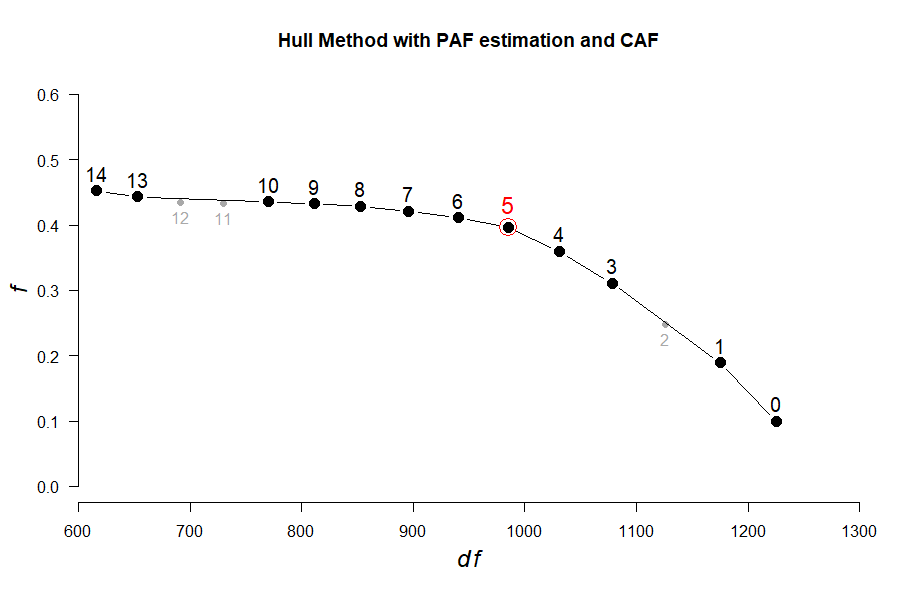
\includegraphics[width=1\linewidth]{04_figures/hull-n-factors} \caption{Results of Kaiser-Guttman criterion for determining the number of factors}\label{fig:hull-figure}
\end{figure}

\begin{figure}
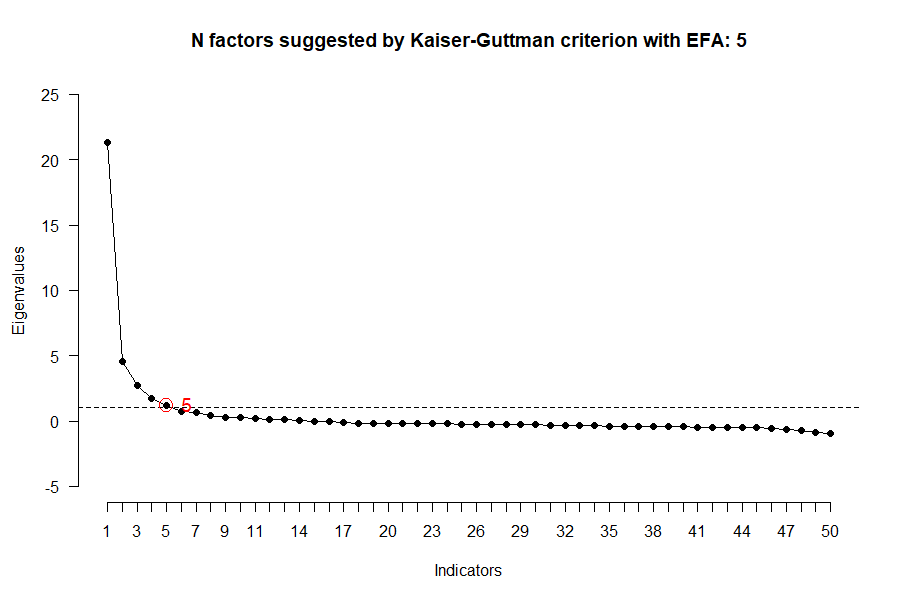
\includegraphics[width=1\linewidth]{04_figures/KGC-n-factors} \caption{Results of Hull method for determining the number of factors}\label{fig:kgc-figure}
\end{figure}

The loadings resulting from the factor analysis are illustrated in
\ref{fig:loading-fig}. We assigned names to each factor based on a visual
inspection of the results. The \emph{drivable} factor had the highest loadings
for variables representing access by car to most destination types. The
\emph{walkable} factor has high loadings for variables representing access
by walking and transit. The \emph{diverse} index is characterized by diversity of
people (high percentages of black residents and low percentages of white
residents), diversity of land use (a greater number of distinct land
uses in the immediate vicinity and a shorter average distance to disamenities),
and lower assessed property values. The \emph{dense} factor is characterized by lower
values for the radius of the smallest buffer containing two thousand residents
(i.e.~higher population densities) and higher access to retail and grocery
locations by non-motorized modes. The \emph{amenities} factor is characterized
by non-motorized and transit access to retail and grocery locations. \ref{fig:loading-fig} illustrates the loadings of each individual variable onto each of the five factors.

\begin{figure}
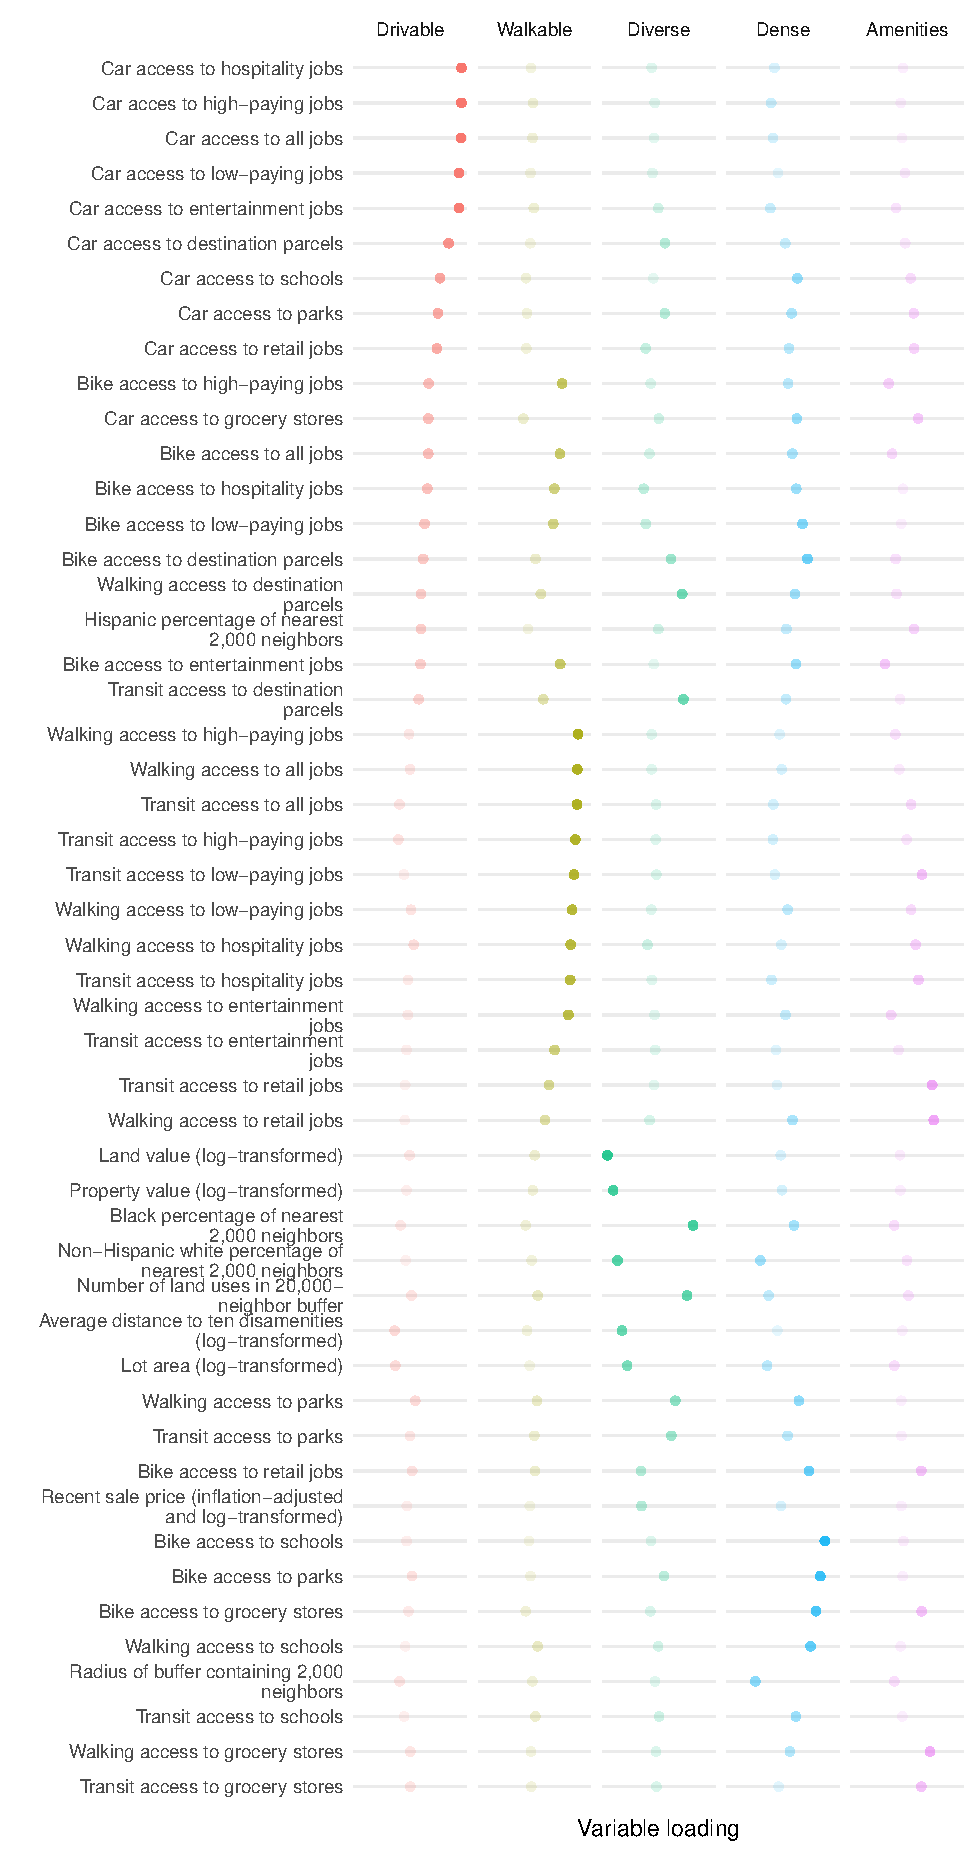
\includegraphics[width=1\linewidth]{_main_files/figure-latex/loading-fig-1} \caption{Factor loadings}\label{fig:loading-fig}
\end{figure}

\ref{fig:drive-map}, \ref{fig:walk-map}, \ref{fig:dense-map},
\ref{fig:diverse-map}, and \ref{fig:amenities-map} show the spatial
variation in the drivability, walkability, density, diversity, and amenity-richness indices, respectively.

\begin{figure}
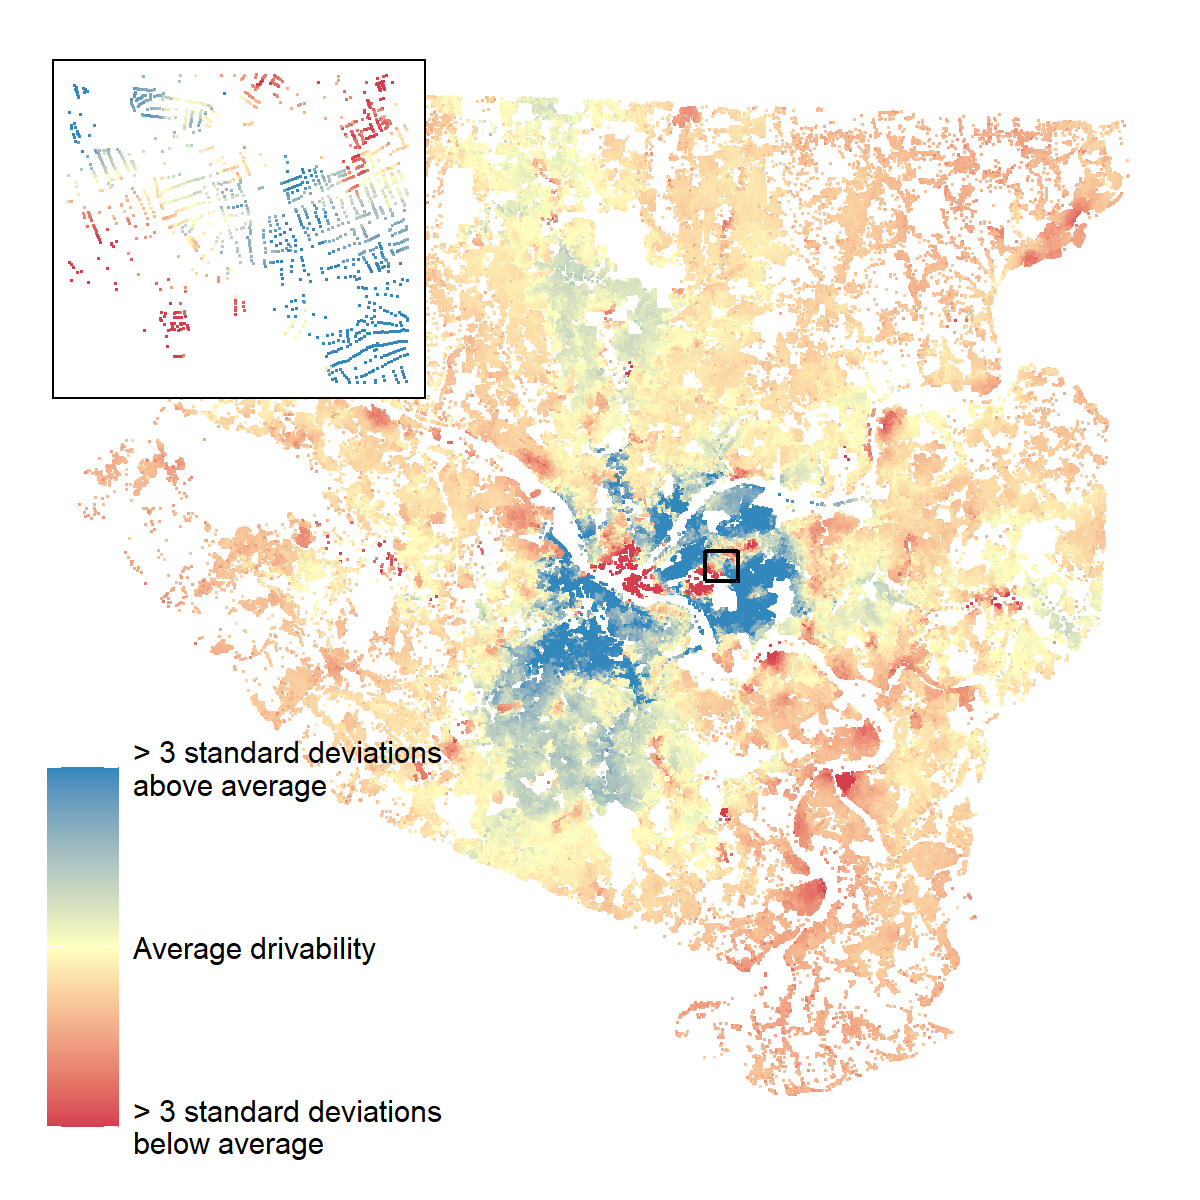
\includegraphics[width=1\linewidth]{04_figures/drivable} \caption{Spatial variation in drivability index}\label{fig:drive-map}
\end{figure}

\begin{figure}
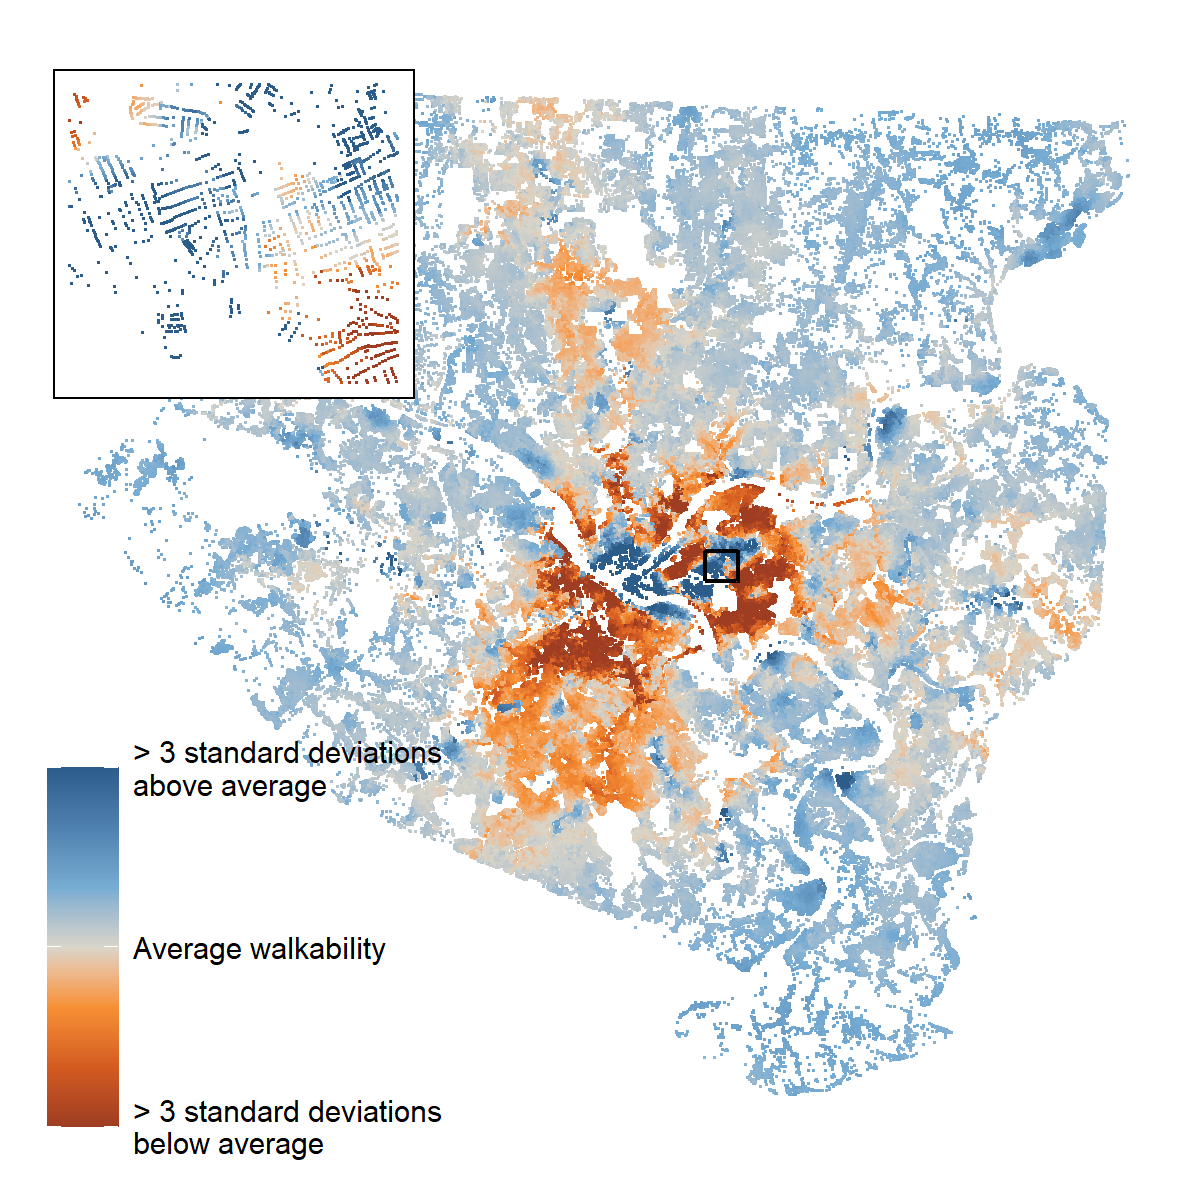
\includegraphics[width=1\linewidth]{04_figures/walkable} \caption{Spatial variation in walkability index}\label{fig:walk-map}
\end{figure}

\begin{figure}
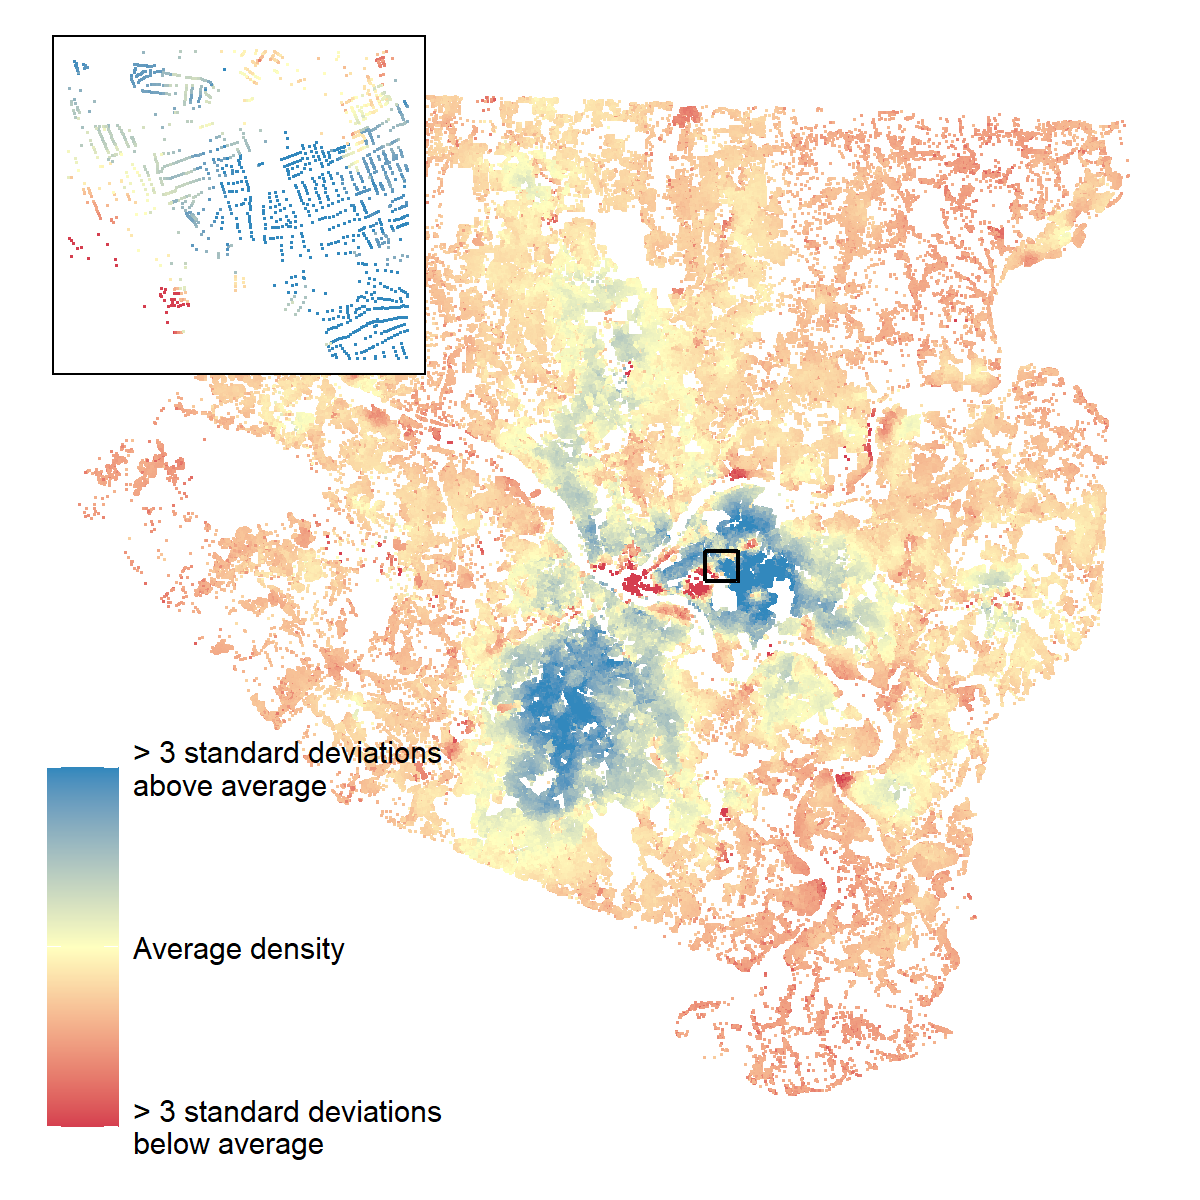
\includegraphics[width=1\linewidth]{04_figures/dense} \caption{Spatial variation in density index}\label{fig:dense-map}
\end{figure}

\begin{figure}
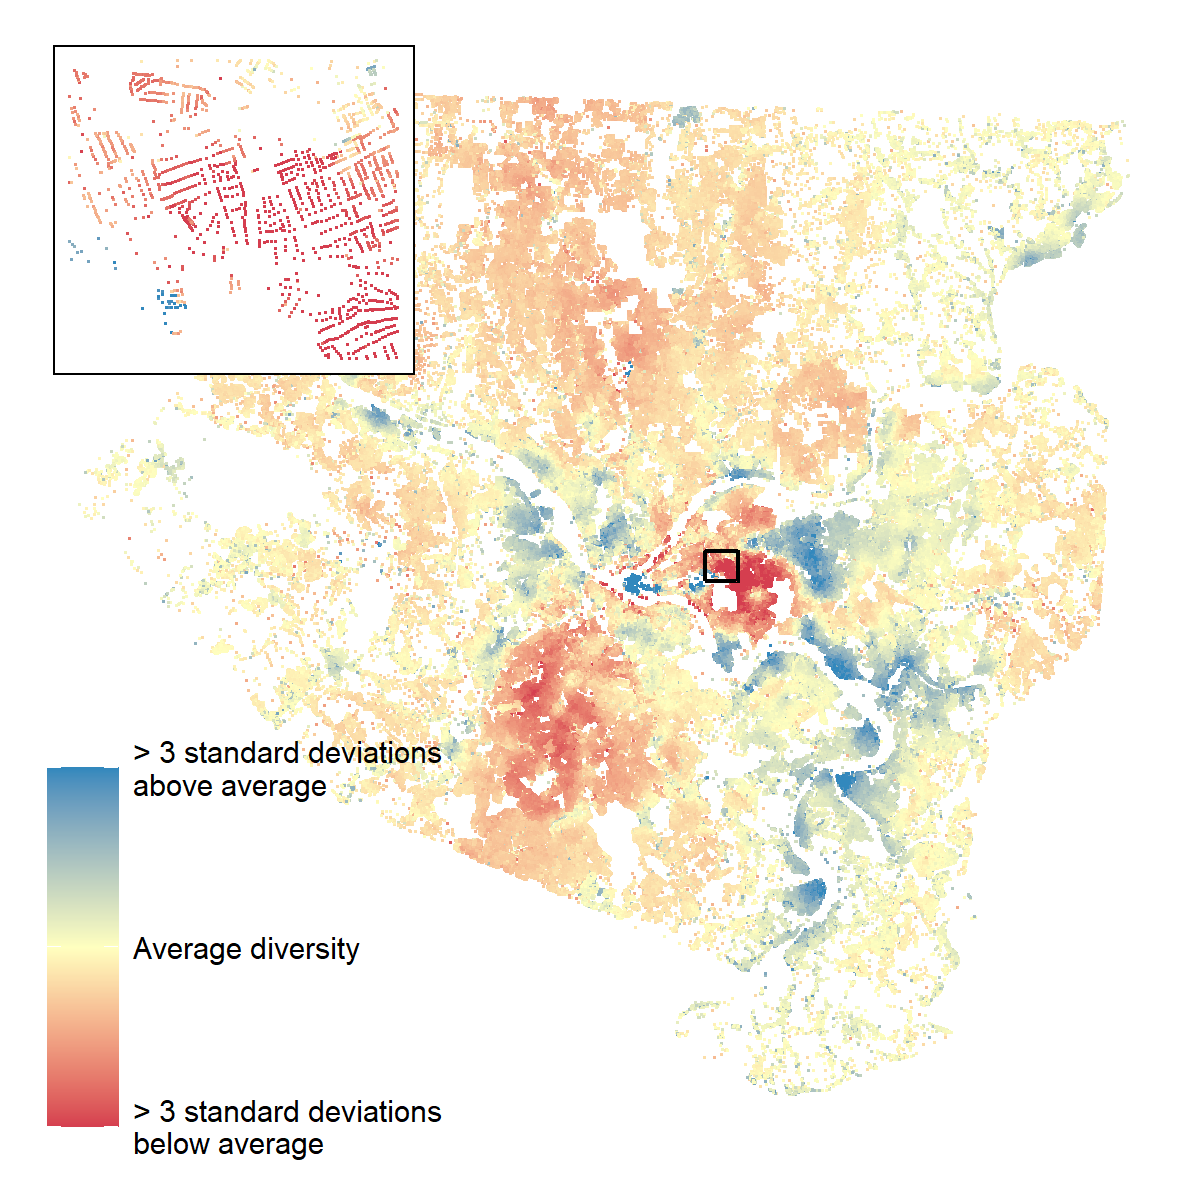
\includegraphics[width=1\linewidth]{04_figures/diverse} \caption{Spatial variation in diversity index}\label{fig:diverse-map}
\end{figure}

\begin{figure}
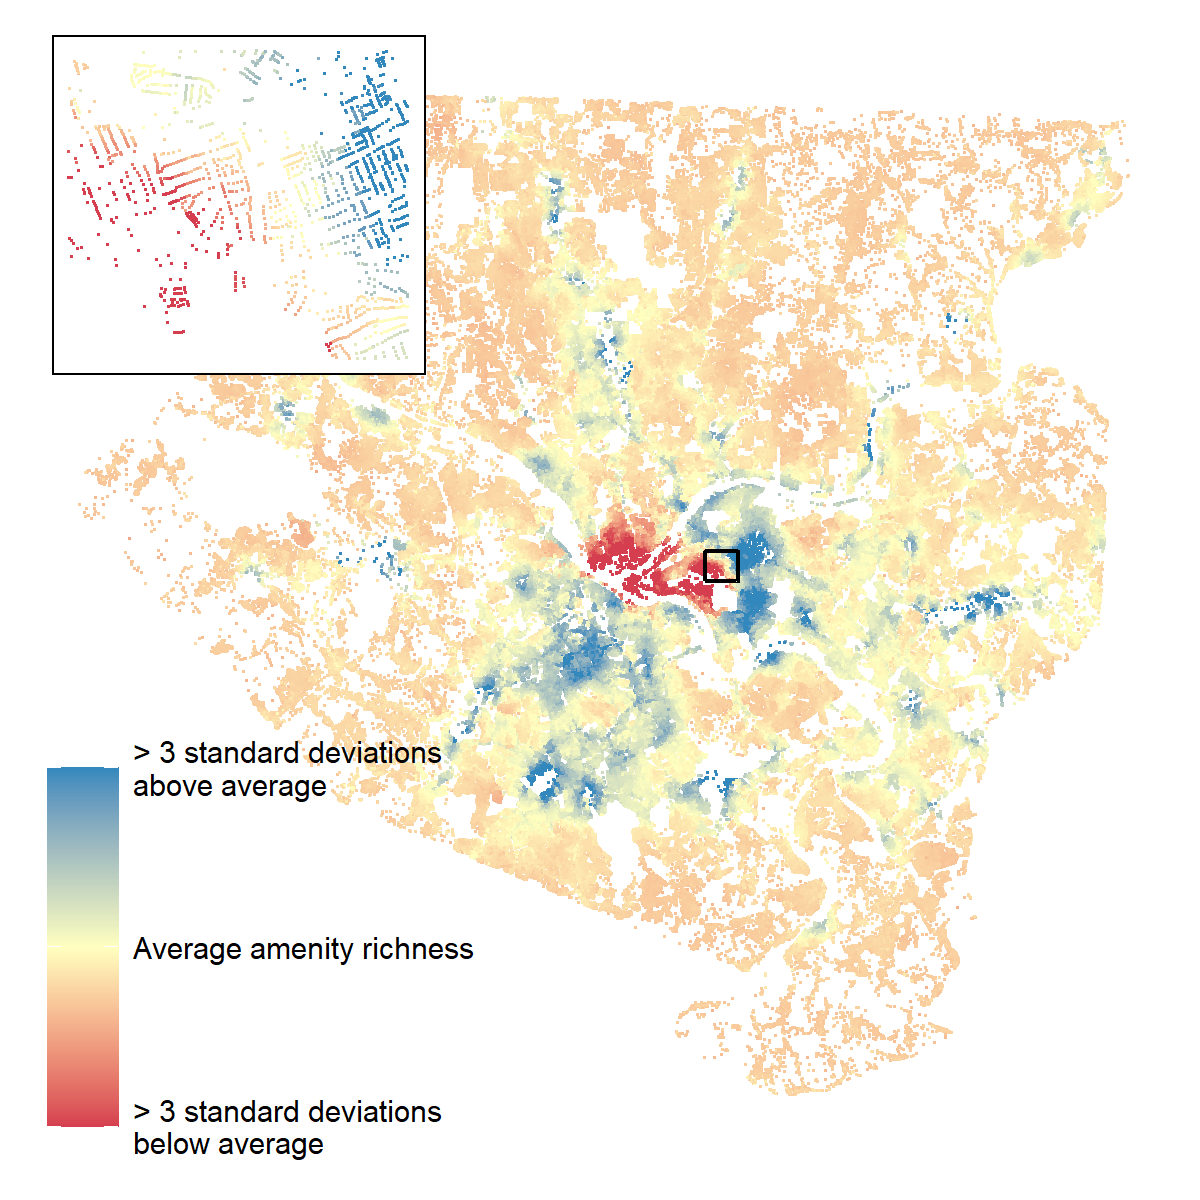
\includegraphics[width=1\linewidth]{04_figures/amenities} \caption{Spatial variation in amenity-richness index}\label{fig:amenities-map}
\end{figure}

\ref{fig:factor-cor} illustrates the distribution of each factor and the
relationships among them.

\begin{figure}
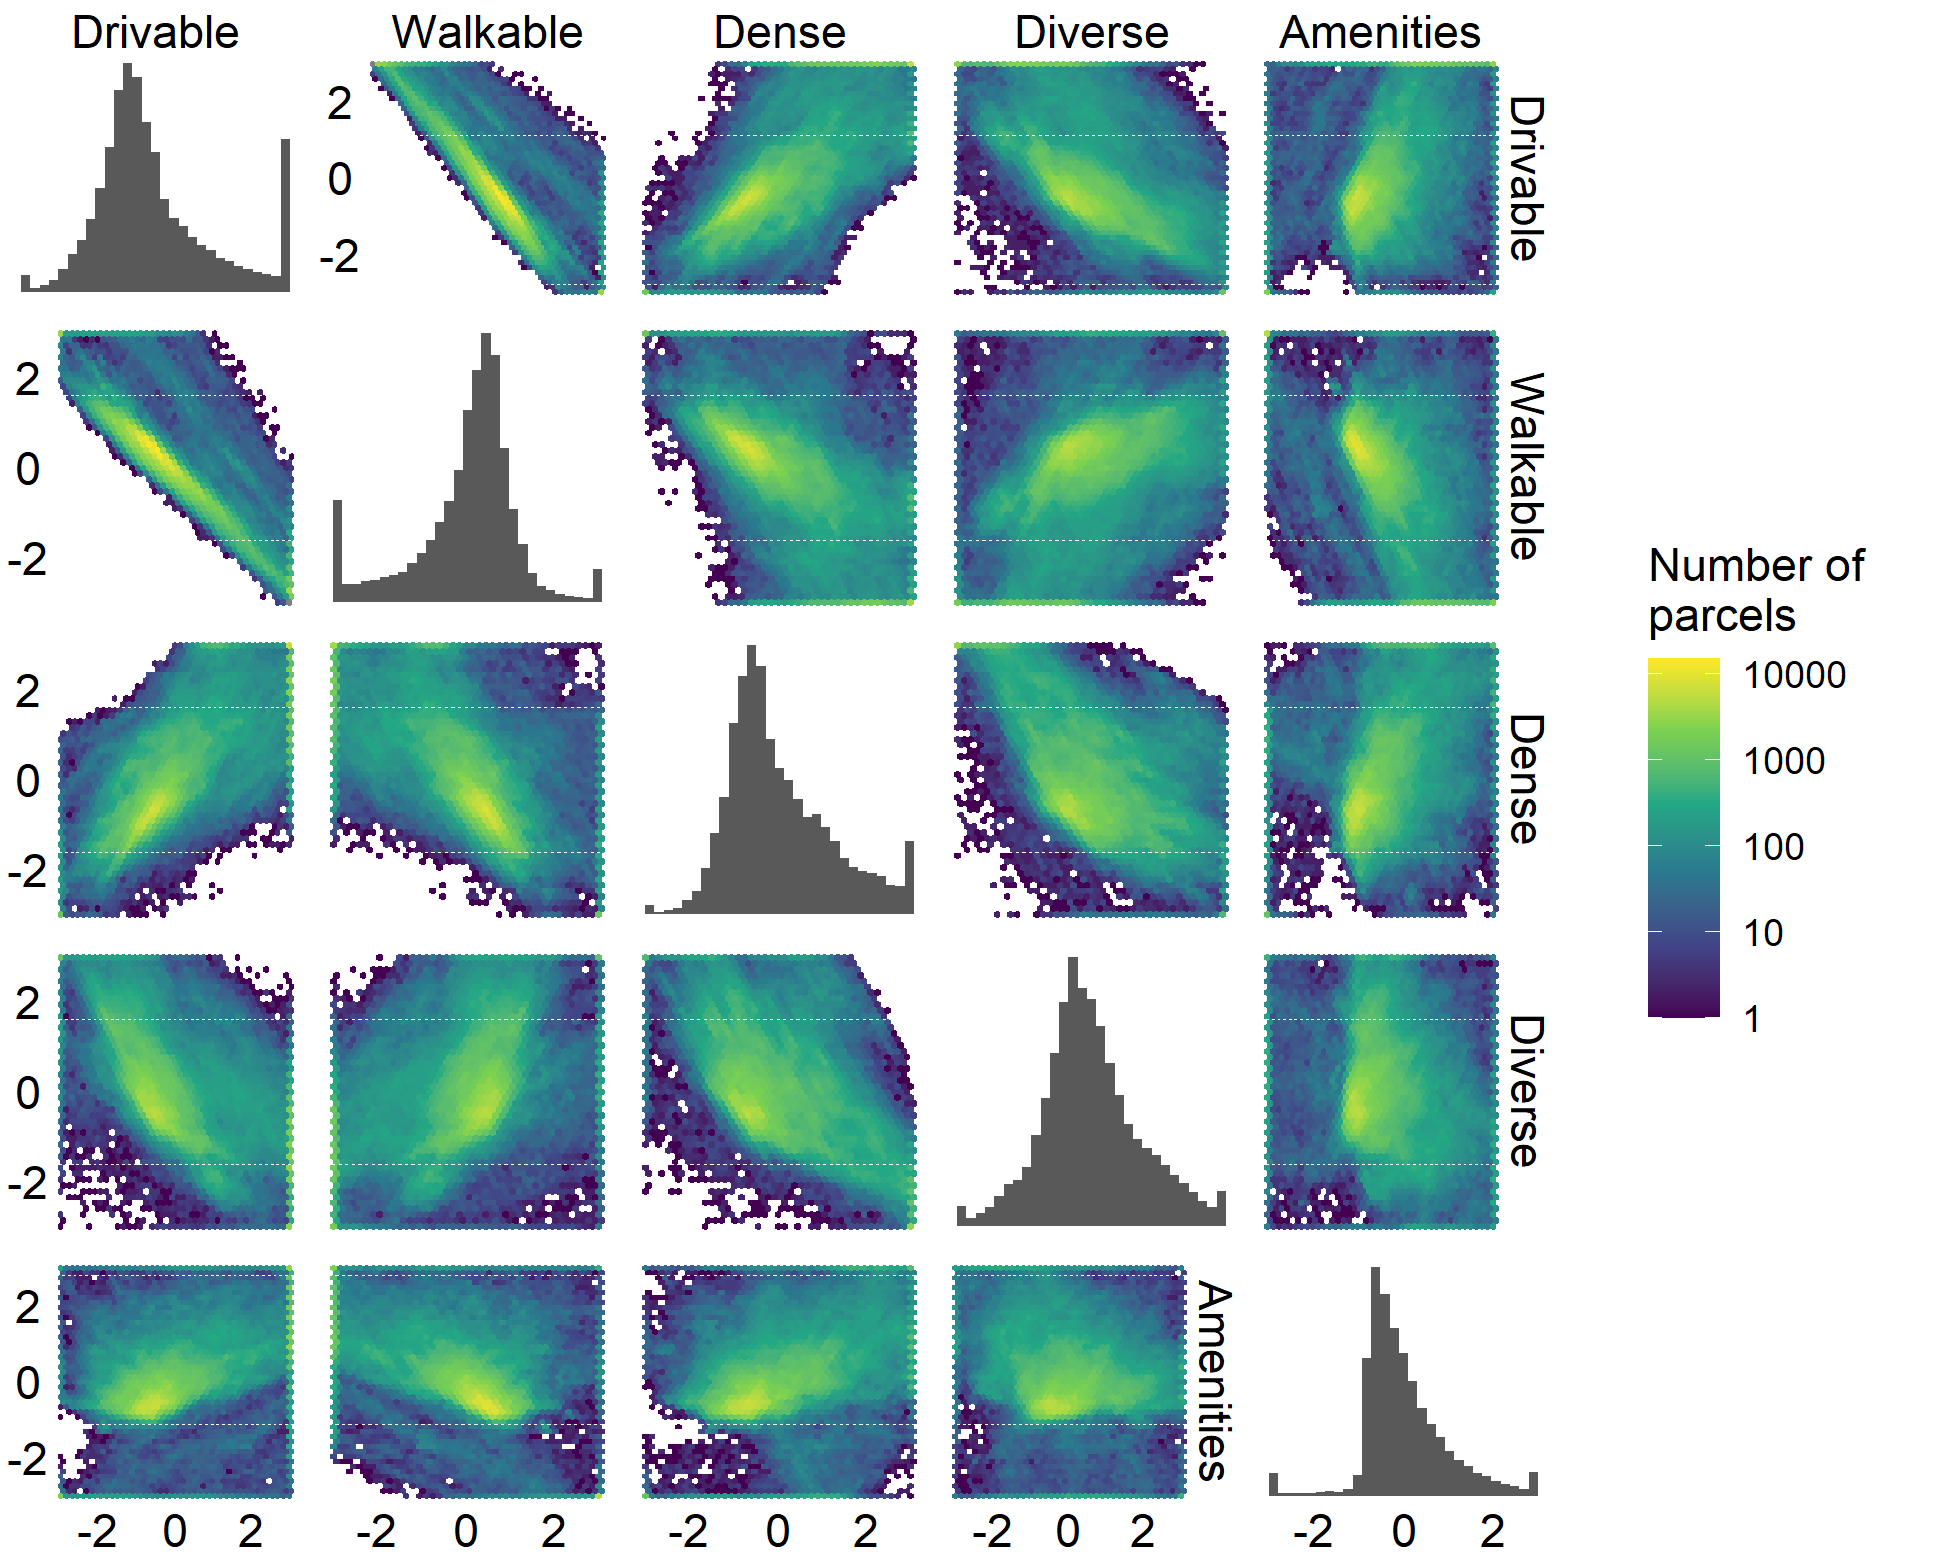
\includegraphics[width=1\linewidth]{04_figures/factor-cor} \caption{Spatial variation in amenity-richness index}\label{fig:factor-cor}
\end{figure}

\hypertarget{implications-for-place-quality}{%
\chapter{Implications for place quality}\label{implications-for-place-quality}}

This would be a good place to discuss the work
with the focus groups.

\hypertarget{sharing-your-book}{%
\chapter{Sharing your book}\label{sharing-your-book}}

\hypertarget{publishing}{%
\section{Publishing}\label{publishing}}

HTML books can be published online, see: \url{https://bookdown.org/yihui/bookdown/publishing.html}

\hypertarget{pages}{%
\section{404 pages}\label{pages}}

By default, users will be directed to a 404 page if they try to access a webpage that cannot be found. If you'd like to customize your 404 page instead of using the default, you may add either a \texttt{\_404.Rmd} or \texttt{\_404.md} file to your project root and use code and/or Markdown syntax.

\hypertarget{metadata-for-sharing}{%
\section{Metadata for sharing}\label{metadata-for-sharing}}

Bookdown HTML books will provide HTML metadata for social sharing on platforms like Twitter, Facebook, and LinkedIn, using information you provide in the \texttt{index.Rmd} YAML. To setup, set the \texttt{url} for your book and the path to your \texttt{cover-image} file. Your book's \texttt{title} and \texttt{description} are also used.

This \texttt{gitbook} uses the same social sharing data across all chapters in your book- all links shared will look the same.

Specify your book's source repository on GitHub using the \texttt{edit} key under the configuration options in the \texttt{\_output.yml} file, which allows users to suggest an edit by linking to a chapter's source file.

Read more about the features of this output format here:

\url{https://pkgs.rstudio.com/bookdown/reference/gitbook.html}

Or use:

\begin{Shaded}
\begin{Highlighting}[]
\NormalTok{?bookdown}\SpecialCharTok{::}\NormalTok{gitbook}
\end{Highlighting}
\end{Shaded}


  \bibliography{book.bib,packages.bib}

\end{document}
